\chapter{緒論}
從1969年網際網路誕生以來,眾多數位化的商品與服務不斷推陳出新,進而大幅改變了人們的生活習慣。然而,貨幣的數位化卻是直到近年來區塊鏈的誕生才得以真正的被實現。良好的數位貨幣系統需要具備下列三特性:
(一)交易紀錄難以被竄改、(二)避免雙花(Double-spending)、(三)避免由某個單一角色控制該數位貨幣系統,下列分別介紹此三項特性。

(一) 交易紀錄難以被竄改:交易紀錄與網路訊息一樣,只是單純的位元碼。如何確定使用者擁有某數位貨幣資產,並保證交易紀錄無法遭人輕易竄改,是非常重要的問題。

(二)避免雙花:在數位貨幣系統中,可能存在同一筆數位資產,因為不當操作而被重複使用的情況,這類問題也被稱之為「雙花問題」。

(三)避免由某個單一角色控制該數位貨幣系統:如果系統中存有一個中央集權的角色,例如:中央政府或金融企業等,來協助交易的清算及交易記錄的保存,那麼前兩項特性是容易被滿足的。這類做法雖然頗具效率,但是賦予單一集權角色過大權力卻可能導致不好的結果。例如:國家能夠透過加印鈔票來稀釋鈔票的價值,進而控制金融市場;遊戲公司也可能透過發行新的虛擬點數,讓原先的虛擬點數一文不值。

區塊鏈便是能同時滿足難以被竄改、無法重複支付且去除中央集權的安全系統。區塊鏈是一種基於分散式系統(Distributed system)的節點備份技術,系統中每一位參與者為稱之為節點。節點間權力相互平等,不需透過中央集權角色來管理系統運作。每一個節點都各自擁有一份帳本資料,節點間會相互溝通合作,來確保所有節點的帳本資料是一致的。因此,攻擊者難以透過攻擊單一節點來癱瘓整個系統運作。在區塊鏈系統裡,所有節點所看到的帳本內容是相同的,帳本內交易順序相同,如此一來節點就能根據帳本內的交易順序了解交易是否生效。
區塊鏈是由連續的區塊所組成,區塊內記錄了節點們所提交的交易內容。區塊之間通過保存哈希值(Hash)實現鏈接。為了增加惡意攻擊難度,區塊內會包含該區塊產生的時間戳(Timestamp)。為了防止惡意節點任意更動過去的帳本資料,每一個區塊會包含一個獨一無二的哈希值,該值是根據前一個區塊的內容所產生的。惡意攻擊者無法任意更動前面的區塊內容。一旦區塊內容改變,哈希值將無法符合,這樣的設計使得區塊鏈變得更加安全。第一個區塊稱為創世區塊(Genesis block),創世區塊是所有區塊中,唯一不需要包含前一個區塊哈希值的特例區塊。
\begin{figure}[!htbp]
\centering
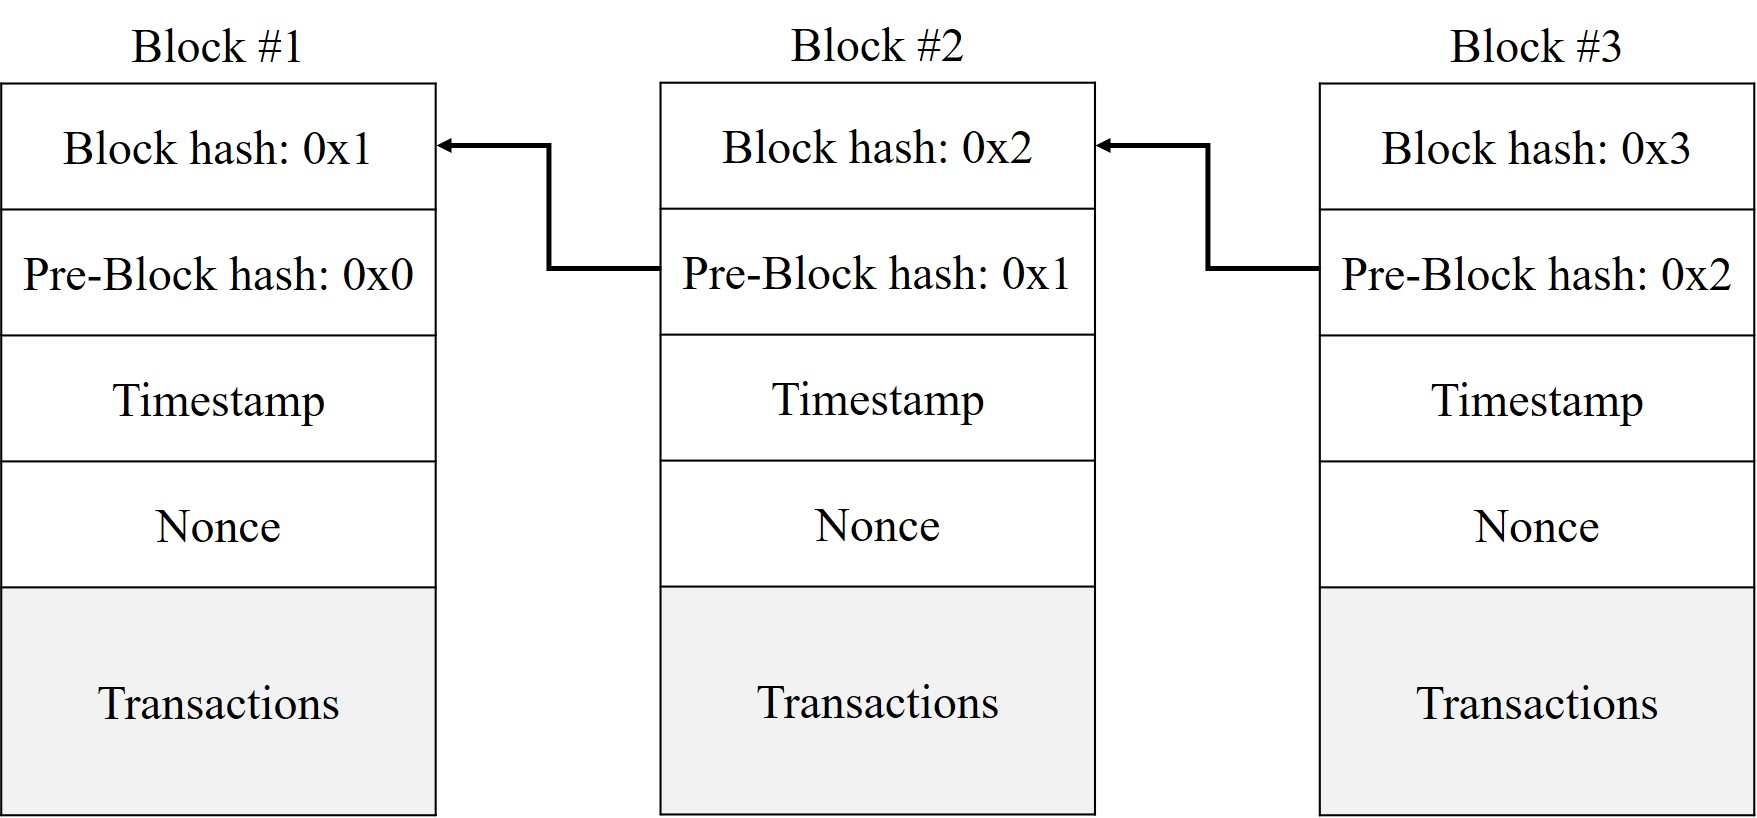
\includegraphics[scale=0.5]{images/1.jpg}
\caption{區塊鏈示意圖}
\label{i:byz-latency}
\end{figure}


因應不同用戶需求及應用場景,區塊鏈系統架構及規模也不盡相同。區塊鏈主要類型可分為公有鏈以及私有鏈。公有鏈的應用如比特幣 \cite{Bitcoin}或以太幣 \cite{Ethereum}等,其特性為任何人都能參與該區塊鏈,加入公有鏈不需要任何人授權,可以隨時自由加入或退出。不同於公有鏈,私有鏈大多是指多個機構共同參與管理的區塊鏈,每個機構執行一個或多個節點,參與私有鏈的節點須有嚴格規範。私有鏈上知名例子包含Facebook Libra \cite{STEVE_HANNA2010}、R3 Corda \cite{R3}等。私有鏈中的資料只允許系統內不同的機構進行讀寫,並且共同記錄及備份資料。由於參與私有鏈的節點是有限制和可控制的,因此私有鏈往往可以有較快的交易速度、更好的隱私保護且不容易被惡意攻擊。本論文將聚焦於私有鏈上。
因為區塊鏈是一個分散式架構,節點間平權管理,所以需要透過運行相同的「共識協議」來維護相同的區塊順序。這類的共識協議則稱為共識演算法。公有鏈上的共識演算法大多採工作量證明(PoW)來達成共識。PoW(Proof-of-Work)透過競賽解題,第一個解出題目的節點將獲得廣播區塊的權力,共識過程中大部分的運算效能都會花在這個解題步驟(俗稱挖礦),因此區塊產出時間會被拉長,導致共識效率低落。然而私有鏈因為節點需經授權才可加入,這類演算法大多透過投票來選擇區塊的廣播者,透過輪流廣播來維持區塊鏈內的平權治理。

私有鏈上通常運行BFT共識演算法,BFT是拜占庭容錯(Byzantine Fault-Tolerant)的縮寫。在拜占庭容錯的區塊鏈上,即使系統中部分節點當機或存在惡意節點情況下,區塊鏈依舊具備安全性(Safety)與活性(Liveness)等性質。安全性能夠保證區塊鏈上每個參與區塊鏈系統的節點,都擁有相同且排序一致的帳本內容。活性則讓區塊鏈是一個永續的系統,能夠容忍錯誤發生且避免因為單一節點故障而導致系統停擺。目前已經有許多BFT共識演算法,傳統的BFT演算法通常需要多個回合才能達成共識。每一個回合會有一個節點擔任提議者(Proposer)。一般來說,一個回合需要執行三個步驟:第一個步驟的目的在於讓提議者廣播其提議,若該提議者廣播多份提議,則區塊鏈可能發生分叉(Fork)進而導致內容衝突。這讓攻擊者可能重複花費同一筆金錢;第二個步驟的目的即為讓所有節點檢查該提議者是否只有廣播一份提議。若提議者只有廣播一份提議,在第三個步驟中,節點便可以開始投票(將收到的提議廣播給其他節點),若一個節點蒐集到足夠多的同意票,該節點便可以確認該提議為最終共識結果;第三個步驟的目的是為了克服訊息傳輸延遲,知名的BFT演算法PBFT \cite{castro1999practical}便是根據上述三個步驟設計。

過去也有少部分的BFT演算法在一個回合中只需要兩個步驟,例子包含FaB \cite{abraham2018revisiting}、Zyzzyva \cite{kotla2007zyzzyva}、SBFT \cite{martin2006fast}、Hydrachain \cite{Hydrachain}。然而,FaB與Zyzzyva已被指出無法保證活性,換句話說,共識演算法可能永遠無法達成共識。另一方面,Hydrachain也被指出無法保證安全性,也就是說,不同的正常節點可能會有不同的共識節果,這在區塊鏈上及代表分岔。雖然SBFT能夠保證安全性與活性,但是SBFT在節點發生故障或是網路延遲過大的情況下,會改用類似PBFT的三步驟設計。因此,在系統狀況良好時,SBFT每回合只需要執行兩個步驟。但是在系統狀況不良時,SBFT每回合仍需要執行三個步驟。
本論文探討的議題為一個新的兩回合拜占庭共識演算法。更明確的說我們希望在不犧牲安全性及活性情況下,設計一個每回合只需要兩個步驟的BFT演算法。重要的是,該BFT演算法即使在系統狀況不佳時,每個回合仍只需要兩個步驟。以下是本篇論本的研究目標: 

\begin{itemize}%项目符号开始
\item 設計一個兩回合的共識演算法-TwoStepBFT並保證安全性及活性。
\item 將TwoStepBFT演算法實作於以太坊(Geth version:1.67)上,並保留以太坊上其他功能。
\item 整合多樣化雲端部署套件,快速在雲端伺服器上建立多台環境一致的機器作為私有鏈共識節點。
\item 自動化生成以太坊節點,將節點部署模組化,讓系統根據使用者需求,快速搭建該私有鏈。
\item 針對不同實驗環境進行效能測試,進行共識效率比較。 
\end{itemize}





